\documentclass[a4paper, fontsize=14pt]{article}
\usepackage[T2A]{fontenc}
\usepackage{mathtools}
\usepackage[utf8]{inputenc}
\usepackage[english, russian]{babel}
\usepackage{fancyhdr}
\usepackage{graphicx}
\usepackage{gensymb}
\usepackage{floatrow}
\usepackage{titlesec}
\usepackage{lastpage}
\usepackage{float}
\usepackage{gensymb}
\usepackage{booktabs}
\usepackage{amsmath}
\usepackage{amssymb}


\pagestyle{fancy}
	\fancyhf{}
	\lhead{\hspace{1bp} Работа \textnumero 3.6.1}
	\rhead{Терехов Максим 876\hspace{1bp}}
	\cfoot{\textbf{}}
	\rfoot{\thepage\ \textnormal{из}\ \pageref{LastPage}}
	\renewcommand{\headrulewidth}{1pt}
	\renewcommand{\footrulewidth}{1pt}


%\addtolength{\hoffset}{-1.75cm}
%\addtolength{\textwidth}{3.5cm} 

%\addtolength{\voffset}{-1.5cm}
%\addtolength{\textheight}{3cm} 

\titleformat{\section}
    [block]{\normalfont\bfseries\large}{\rlap{\thesection}}{0em}
    {\vspace{-0.02\textwidth}\begin{minipage}[t]{.95\textwidth}}
[\end{minipage}]

\thispagestyle{fancy}

\begin{document}
\selectlanguage{russian}



\huge
\centering
\textbf{Спектральный анализ электрических сигналов}

\raggedright
\large
\parindent=1cm
\section*{Цель работы}
Изучение спектрального состава периодических электрических сигналов
\section*{Оборудование}
Анализатор спектра, генератор прямоугольных импульсов, генератор сигналов специальной формы, осциллограф.
\section*{Экспериментальная установка}
\begin{figure}[H]
\center
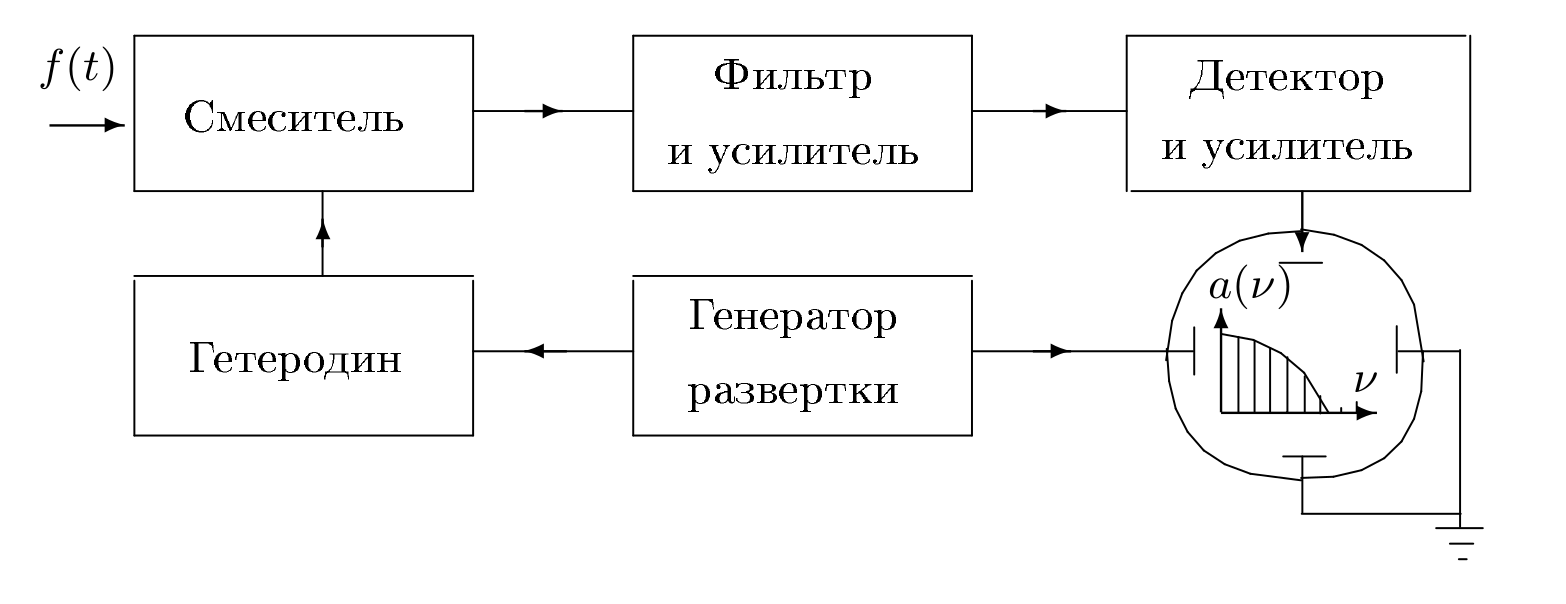
\includegraphics[scale=0.2]{ust.png}
\caption{Структурная схема анализатора спектра}
\end{figure}
\begin{figure}[H]
\center
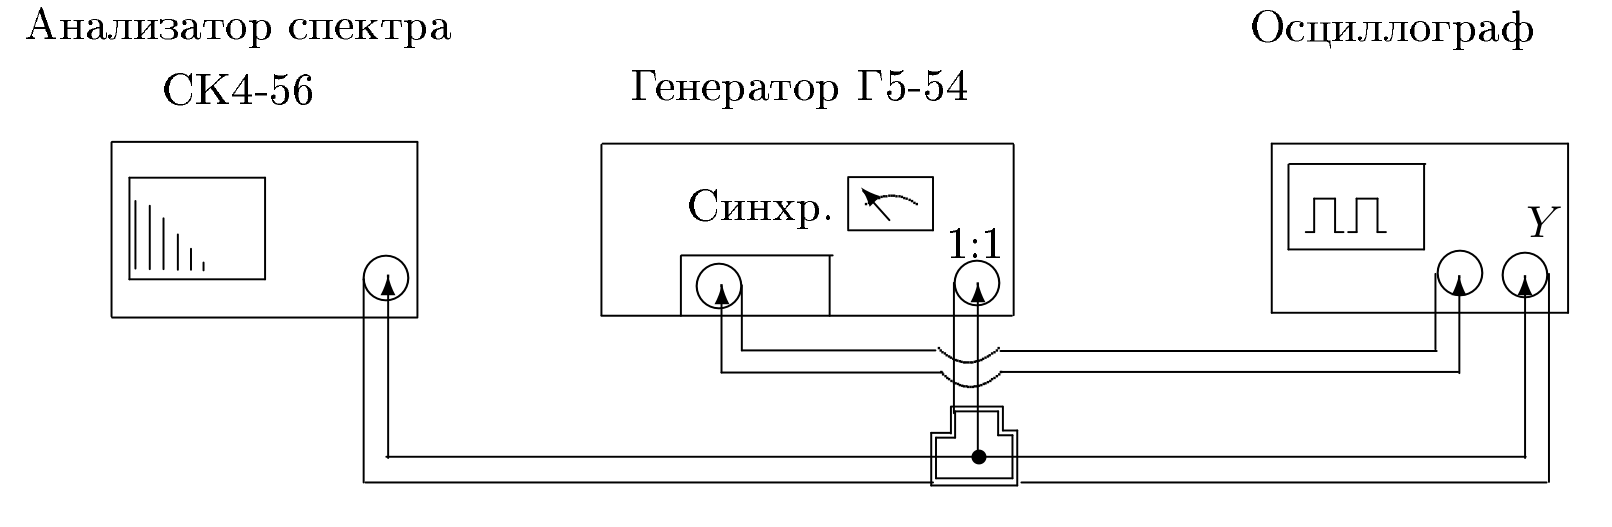
\includegraphics[scale=0.2]{ust1.png}
\caption{Схема для исследования спектра периодической последовательности прямоугольных импульсов}
\end{figure}
\begin{figure}[H]
\center
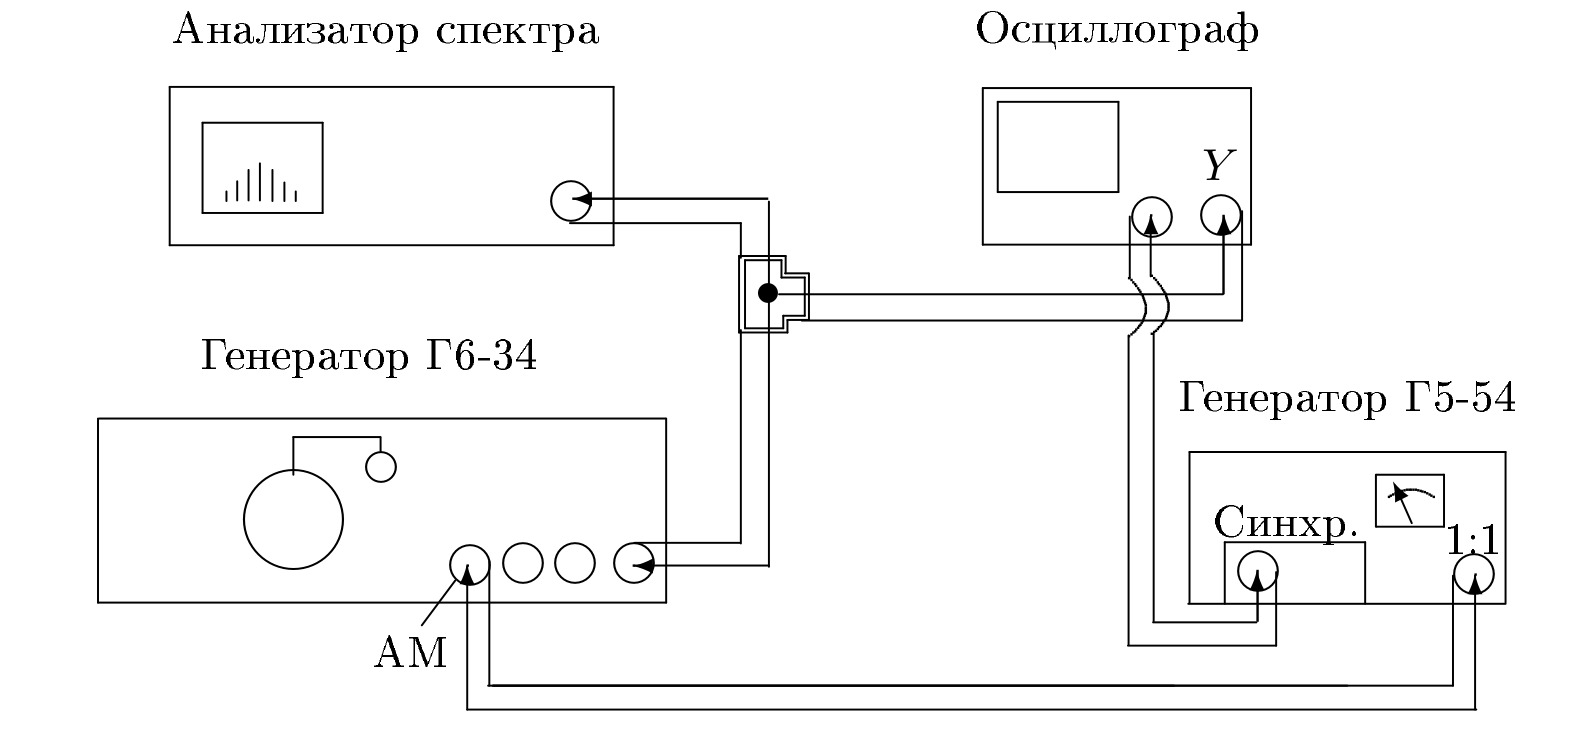
\includegraphics[scale=0.2]{ust2.png}
\caption{Схема для исследования спектра периодической последовательности цугов высокочастотных колебаний}
\end{figure}
\begin{figure}[H]
\center
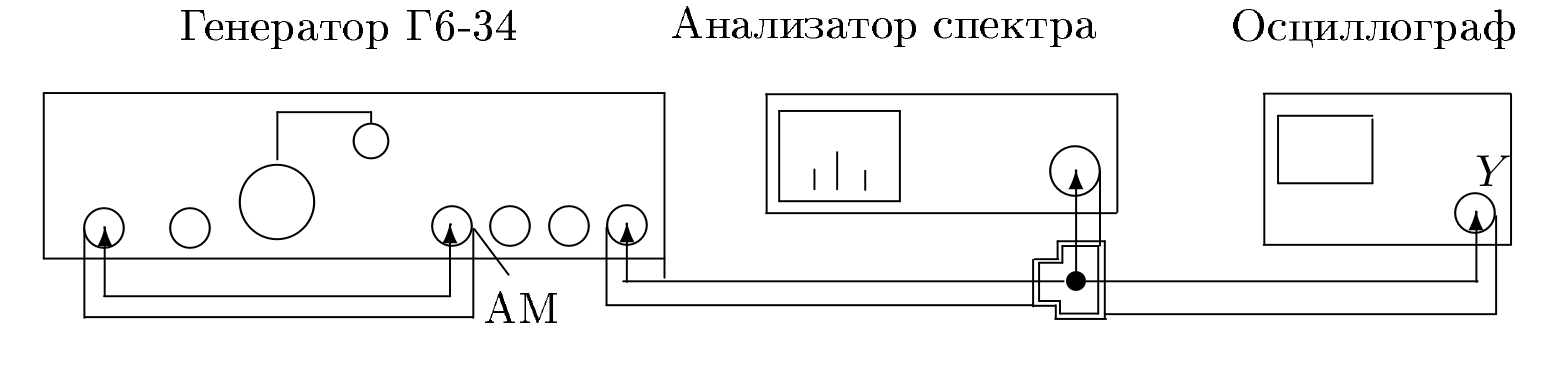
\includegraphics[scale=0.2]{ust3.png}
\caption{Схема для исследования спектра высокочастотного гармонического сигнала, промодулированного по амплитуде низкочастотным гармоническим сигналом}
\end{figure}
\section*{Теоретическая часть}
Рассмотрим функцию вида 
\[
	f(t)=A_{1} \cos \left(\omega_{1} t-\alpha_{1}\right)+A_{2} \cos \left(\omega_{2} t-\alpha_{2}\right)+\ldots+A_{N} \cos \left(\omega_{N} t-\alpha_{N}\right),
\]
или в более короткой записи
\[
	f(t)=\sum_{n=1}^{N} A_{n} \cos \left(\omega_{n} t-\alpha_{n}\right),
\]
где $A_n, \omega_n, \alpha_n$ --- постоянные величины. Множество пар $(\omega_1, A_1), (\omega_2, A_2), \ldots, (\omega_n, A_n)$ называется спектром функции $f(t)$. $N$ может быть конечным или бесконечным.

В физике широко используется разложение сложных сигналов на гармонические колебания различных частот $\omega$. Представление периодического сигнала в виде суммы гармонических сигналов в математике называется разложением в ряд Фурье. Непериодические сигналы представляются в виде интеграла Фурье.
\begin{figure}[H]
\center
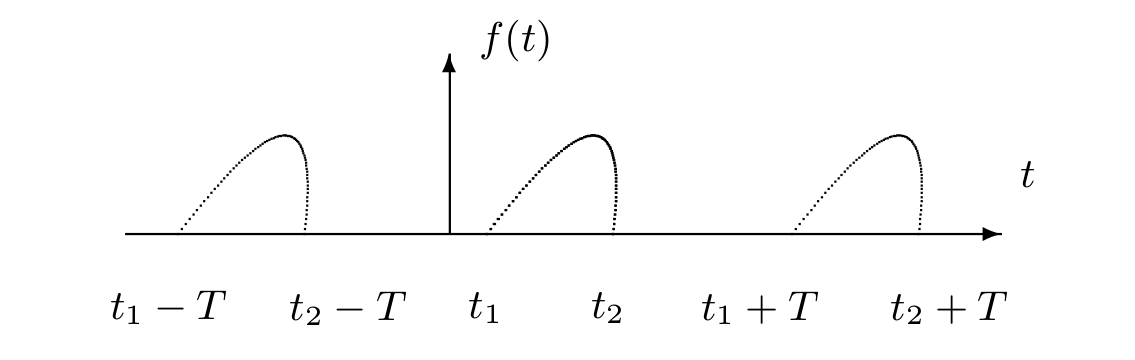
\includegraphics[scale=0.3]{gr0.png}
\caption{График периодической функции с периодом повторения $T$}
\end{figure}
Пусть заданная функция $f(t)$ периодически повторяется с частотой $\Omega_1 = 2 \pi / T$, где $T$ --- период повторения. Её разложение в ряд Фурье имеет вид
\[
f(t)=\frac{a_{0}}{2}+\sum_{n=1}^{\infty}\left[a_{n} \cos \left(n \Omega_{1} t\right)+b_{n} \sin \left(n \Omega_{1} t\right)\right],
\]
или
\[
	f(t)=\frac{a_{0}}{2}+\sum_{n=1}^{\infty} A_n \cos (n \Omega_1 t - \psi_n).
\]
Здесь $a_0 / 2$ --- постоянная составляющая (среднее значение) функции $f(t)$; $a_n$ и $b_n$ --- коэффициенты косинусных и синусных членов разложения. Они определяются выражениями
\[
		a_{n}=\frac{2}{T} \int\limits_{t_{1}}^{t_{1}+T} f(t) \cos \left(n \Omega_{1} t\right) d t;
\]
\[
b_{n}=\frac{2}{T} \int\limits_{t_{1}}^{t_{1}+T} f(t) \sin \left(n \Omega_{1} t\right) d t
\]
Точку начала интегрирования $t_1$ можно выбрать произвольно.

В тех случаях, когда сигнал чётен относительно $t = 0$, так что $f(t) = f(-t)$, в тригонометрической записи остаются только косинусные членыЮ так как все коэффициенты $b_n$ обращаются в нуль. Для нечётной относительно $t = 0$ функции, наоборот, в нуль обращаются коэффициенты $a_n$, и ряд состоит только из синусных членов.

Амплитуда $A_n$ и фаза $\psi_n$ $n$-й гармоники выражаются через коэффициенты $a_n$ и $b_n$ следующим образом:
\[
	A_n = \sqrt{a_n^2 + b_n^2}; \quad \psi_n = \arctg \frac{b_n}{a_n}.
\]
Заменим косинусы экспонентами в соответствии с формулой
\[
	\cos \alpha = \frac{e^{i \alpha} + e^{-i \alpha}}{2}.
\]
Подстановка даёт
\[
f(t)=\frac{1}{2}\left(a_{0}+\sum_{n=1}^{\infty} A_{n} e^{-i \psi_{n}} e^{i n \Omega_{1} t}+\sum_{n=1}^{\infty} A_{n} e^{i \psi_{n}} e^{-i n \Omega_{1} t}\right).
\]
Введём комплексные амплитуды $\hat A_n$ и $\hat A_{-n}$:
\[
	\hat A_n = A_n e^{i \psi_n}; \quad \hat A_{-n} = A_n e^{i \psi_n}; \quad \hat A_0 = a_0.
\]
Разложение $f(t)$ приобретает вид
\[
	f(t) = \frac{1}{2} \sum_{n = - \infty}^{\infty} \hat A_n e^{i n \Omega_1 t}.
\]
Таким образом, введение отрицательных частот (типа $-n\Omega_1$) позволяет записать разложение Фурье особенно простым образом. Формулы комплексных амплитуд обеспечивают действительность суммы: в каждой частоте $k \Omega_1$ соответствуют один член из разложение в ряд Фурье до комплексных амплитуд ($n = k$), а в разолжении суммы --- два члена ($n = k$ И $n = -k$). Формулы комплексных амплитуд позволяют переходить от действительного разложения к комплексному и обратно.

Для расчёта комплксных амплитуд $A_n$ не обязательно пользоваться формулами комплексных амплитуд, полученных выше. Умножим левую и правую части разложения в сумму с комплексными амплитудами на $e^{-i k \Omega_1 t}$ и проинтегрируем полученное равенство по времени на отрезке, равном одному периоду, например, от $t_1 = 0$ до $t_2 = 2 \pi / \Omega_1$. В правой части обратятся в нуль все члены, кроме одного, соответствующего $n = k$. Этот член даёт $A_k T /2$. Имеем поэтому
\[
	\hat A_k = \frac{2}{T} \int\limits_0^T f(t) e^{-i k \Omega_1 t} dt.
\]
Как мы видим, спектр любой периодической функции состоит из набора гармонических колебаний с дискретными частотами: $\Omega_1, 2\Omega_1, 3\Omega_1, \ldots$ и постоянной составляющей, которую можно рассматривать как колебание с нулевой частотой $(0 \cdot \Omega_1)$. Такой спектр называют линейчатым или дискретным.

Пусть непериодический сигнал $f(t)$ действует в конечно временном интервале $t_1 < t < t_2$. Превратим функцию $f(t)$ в периодическую путём повторения её с произвольным периодом $T > (t_1 - t_2)$. Для этой новой функции применимо разложение в ряд Фурье. В соответствии с формулами абсолютная величина коэффициентов $a_n$ и $b_n$ обратно пропорциональна $T$, поэтому устремляя $T$ к бесконечности, в пределе получим бесконечно малые амплитуды гармонических составляющих. Количество составляющих, входящих в ряд Фурье, будет при этом бесконечно большим, так как при $T \rightarrow \infty$ частота $\Omega_1 = \frac{2 \pi}{T} \rightarrow 0$. Другими словами, расстояние между спектральными линиями, равное частоте $\Omega_1$, становится бесконечно малым, и спектр из дискретного переходит в сплошной.

Воспольхуемся комплексной формулой ряда Фурье и подставим вместо $A_n$ выражение:
\[
	\begin{aligned} f(t)=\sum_{n \rightarrow-\infty}^{+\infty} \frac{1}{T} & \left[\int_{t_{1}}^{t_{2}} f(t) e^{-i n \Omega_{1} t} d t\right]  e^{i n \Omega_{1} t}=\\=& \frac{1}{2 \pi} \sum_{n \rightarrow-\infty}^{+\infty} \frac{1}{T}\left[\int_{t_{1}}^{t_{2}} f(t) e^{-i n \Omega_{1} t} d t\right] e^{i n \Omega_{1} t} \cdot \Omega_{1}. \end{aligned}
\]
При записи второго выражения использована связь $T = 2 \pi / \Omega_1$.

При $T \rightarrow \infty$ частота $\Omega_1$ превращается в $d \Omega_1$, $n \Omega_1$ --- в текущую частоту $\Omega$, а операция суммирования --- в операцию интегрирования. В результате получаем двойной интеграл Фурье:
\[
f(t)=\frac{1}{2 \pi} \int_{-\infty}^{\infty}\left[\int_{t_{1}}^{t_{2}} f(t) e^{-i \Omega t} d t\right] e^{i \Omega t} d \Omega.
\]
Внутренний интеграл обозначим
\[
\hat F(\Omega) = \int\limits_{t_1}^{t_2} f(t) e^{-i \Omega t} dt.
\]
$\hat F(\Omega)$ называется спектральной плотностью или спектральной характеристикой функции $f(t)$. Сравнивая полченное выражение с предыдущим для комплексной амплитуды соответствующеей гармоники ($\Omega = \Omega_n$) той же самой функции, но уже периодической, получим
\[
	2 \hat F(\Omega_n) = T \cdot \hat A_n = 2 \pi \frac{\hat A_n}{\Omega_1}.
\]
Поскольку $\Omega_1$ --- это полоса частот, определяющая соседние спектральные линии дискретного спектра, то $\hat F(\Omega)$ имеет смысл плотности амплитуд.

Из вышееречисленного соотношения следует важный вывод: огибающая сплошного спектра непериодической функции и огибающая линейчатого спектра той же периодической функции совпадают по форме и отличаются только масштабом.

\textbf{Примеры спектров периодических функций}
\begin{figure}[H]
\center
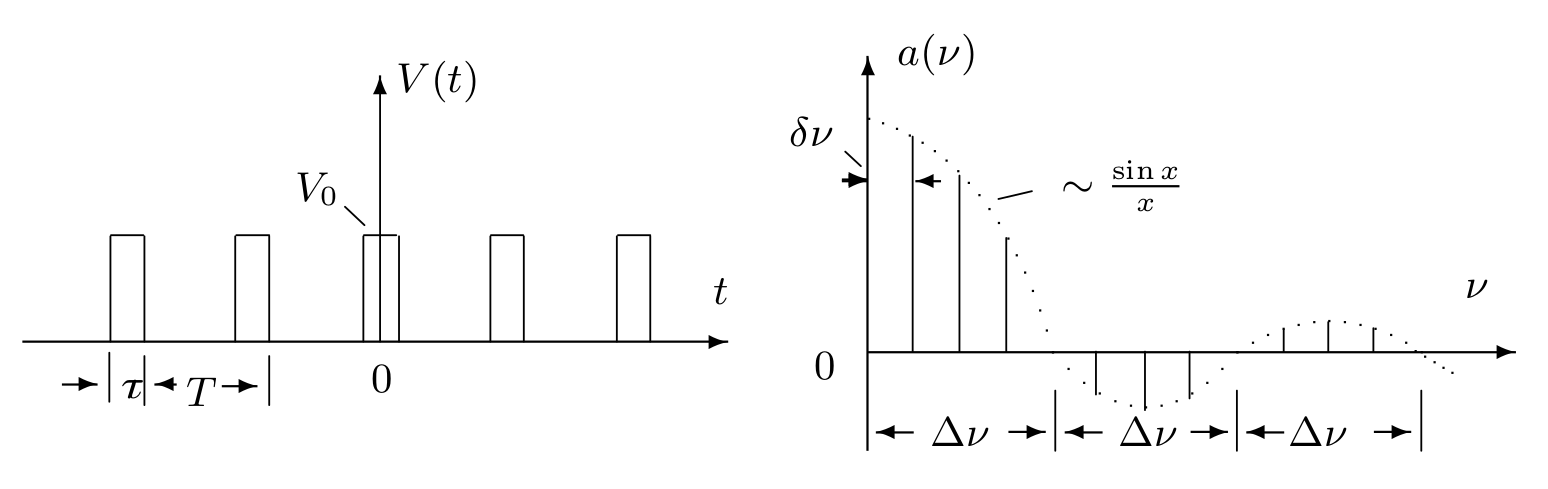
\includegraphics[scale=0.2]{gr1.png}
\caption{Периодическая последовательность прямоугольных импульсов и её спектр}
\end{figure}

Периодическая последовательность прямоугольных импульсов с амплитудой $V_0$, длительностью $\tau$, частотой повторения $\Omega_1 = 2 \pi / T$, где $T$ --- период повторения импульсов.

Найдём среднее значение (постоянную составляющую):
\[
	\langle V\rangle=\frac{a_{0}}{2}=\frac{A_{0}}{2}=\frac{1}{T} \int\limits_{-\tau / 2}^{\tau / 2} V_{0} d t=V_{0} \frac{\tau}{T}
\]
Коэффициенты при косинусных составляющих равны 
\[
	a_n = \frac{2}{T} \int\limits_{-\tau/2}^{\tau/2} V_0 \cos (n \Omega_1 t) dt = 2 V_0 \frac{\tau}{T} \frac{\sin (n \Omega_1 \tau / 2)}{n \Omega_1 \tau / 2} \sim \frac{\sin x}{x}.
\]
Поскольку наша функция чётная, все коэффициенты синусоидальных гармоник $b_n = 0$. Спектр $a_n$ последовательности прямоугольных импульсов представлен на рисунке. Амплитуды гармоник $A_n (A_n = |a_n|)$ меняются по закону $|\sin x / x|$.

На рисунке изображён случай, когда $T$ кратно $\tau$. Назовём шириной спектра $\Delta \omega$ (или $\Delta \nu = \Delta \omega / 2 \pi$) расстояние от главного максимума ($\omega = 0$) до первого нуля огибающей, возникающего, как нетрудно убедиться, при $n = 2 \pi / \tau \Omega_1$. При этом
\[
	\Delta \omega \tau \simeq 2 \pi \quad \text{или} \quad \Delta \nu \Delta t \simeq 1.
\]
Полученное соотношение взаимной связи интервалов $\Delta \nu$ и $\Delta t$ является частным случаем соотношения неопределённости в квантовой механике. Несовместимость острой локализации волнового процесса во времени с узким спектром частот --- явление широко известное в радиотехнике. Ширина селективной настройки $\Delta \nu$ радиоприёмника ограничивает приём радиосигналов длительность. $t < 1 / \Delta \nu$.

\begin{figure}[H]
\center
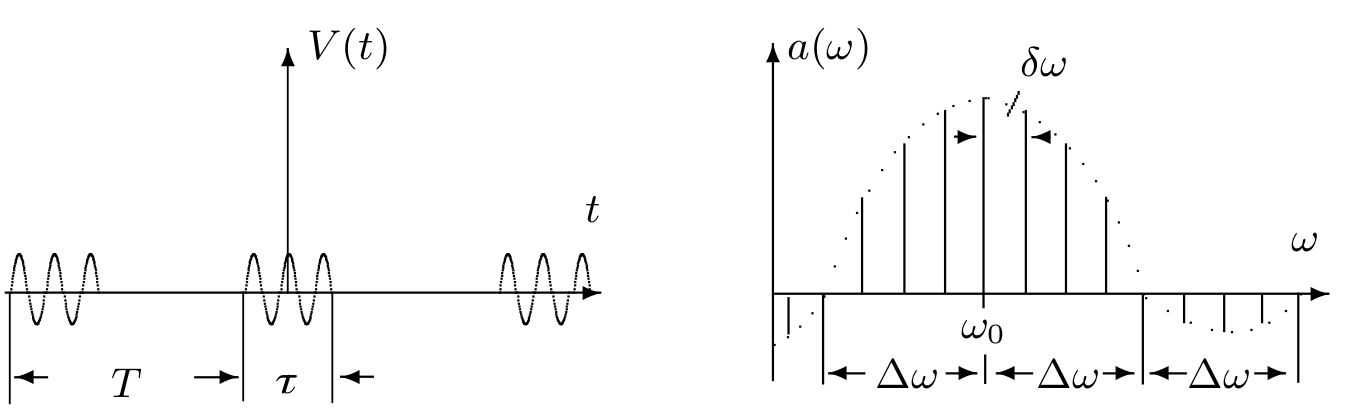
\includegraphics[scale=0.2]{gr2.png}
\caption{Периодическая последовательность цугов и её спектр}
\end{figure}
Периодическая последовательность цугов гармонического колебания $V_0 \cos (\omega_0 t)$ с длительностью цуга $\tau$ и периодом повторения $T$. Функция $f(t)$ снова является чётной относительно $t = 0$. Коэффициент при $n$-й гармонике согласно формуле равен
\[
\begin{aligned} a_{n}=\frac{2}{T} & \int_{-\tau / 2}^{\tau / 2} V_{0} \cos \left(\omega_{0} t\right) \cdot \cos \left(n \Omega_{1} t\right) d t=\\=& V_{0} \frac{\tau}{T}\left(\frac{\sin \left[\left(\omega_{0}-n \Omega_{1}\right) \frac{\tau}{2}\right]}{\left(\omega_{0}-n \Omega_{1}\right) \frac{\tau}{2}}+\frac{\sin \left[\left(\omega_{0}+n \Omega_{1}\right) \frac{\pi}{2}\right]}{\left(\omega_{0}+n \Omega_{1}\right) \frac{\pi}{2}}\right) \end{aligned}.
\]
Зависимость для случая, когда $T / \tau$ равно целому числу, представлена на рисунке выше. Сравнивая спектр последовательности прямоугольных импульсов и спектр цугов, мы видим, что они аналогичны, но их максимумы сдвинуты по частоте на величину $\omega_0$.

\begin{figure}[H]
\center
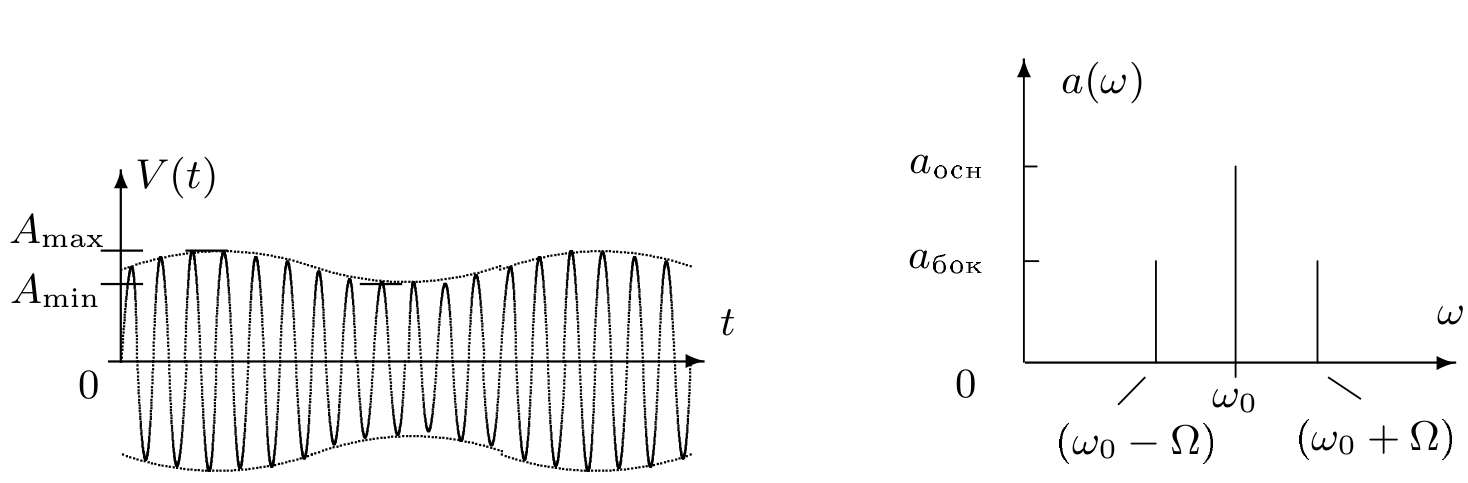
\includegraphics[scale=0.2]{gr3.png}
\caption{Гармонические колебания, модулированные по амплитуде и их спектр}
\end{figure}
Рассмотрим гармонические колебания высокой частоты $\omega_0$, амплитуда которых медленно меняется по гармоническому закону с частотой $\Omega (\Omega \ll \omega_0)$:
\[
	f(t) = A_0 [1 + m \cos \Omega t] \cos \omega_0 t.
\]
Коэффициент $m$ называют глубиной модуляции. При $m < 1$ амплитуда колебаний меняется от минимальной $A_{min} = A_0 (1 - m)$ до максимальной $A_{max} = A_0 (1 + m)$. Глубина модуляции может быть представлена в виде
\[
	m = \frac{A_{max} - A_{min}}{A_{max} + A_{min}}.
\]
Простым тригонометрическим преобразованием уравнения можно найти спектр амплитудно-модулированных колебаний:
\[
\begin{array}{c}{f(t)=A_{0} \cos \left(\omega_{0} t\right)+A_{0} m \cos (\Omega t) \cos \left(\omega_{0} t\right)=} \\ {=A_{0} \cos \left(\omega_{0} t\right)+\frac{A_{0} m}{2} \cos \left(\omega_{0}+\Omega\right) t+\frac{A_{0} m}{2} \cos \left(\omega_{0}-\Omega\right) t}\end{array}
\].
Спектр таких колебаний содержит три составляющих --- основную компоненту и две боковых. Первое слагаемое в правой части представляет собой исходное немодулированное колебание с основной (несущей) частотой $\omega_0$ и амплитудой $a_\text{осн} = A_0$. Второе и третье слагаемые соответствуют новым гармоническим колебаниям с частотами $(\omega_0 + \Omega)$ и $(\omega_0 - \Omega)$. Амплитуды этих двух колебаний одинаковы и составляют $m / 2$ от амплитуды немодулированного колебания: $a_\text{бок} = A_0 m / 2$. Начальные фазы трёх колебаний одинаковы.
\newpage
\section*{Обработка результатов экспериментов}
\textbf{Исследование спектра периодической последовательности прямоугольных импульсов:}1
\begin{figure}[H]
\center
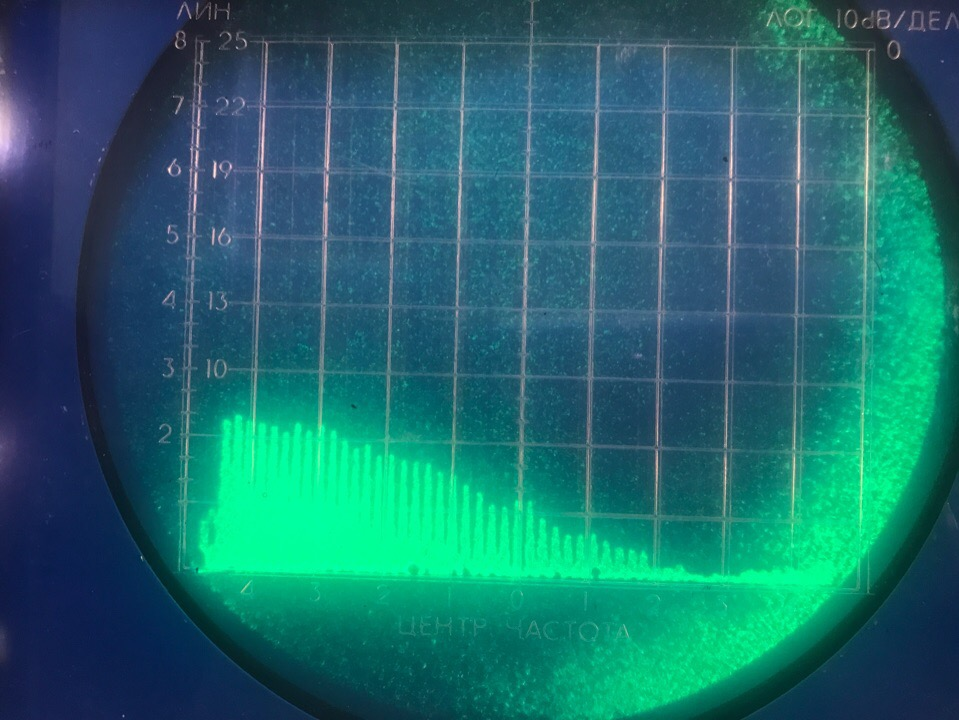
\includegraphics[scale=0.3]{1.jpg}
\caption{Спектр прямоугольных импульсов при $f_\text{повт} = 1$ кГц и $\tau = 25$ мкс}
\end{figure}
\begin{figure}[H]
\center
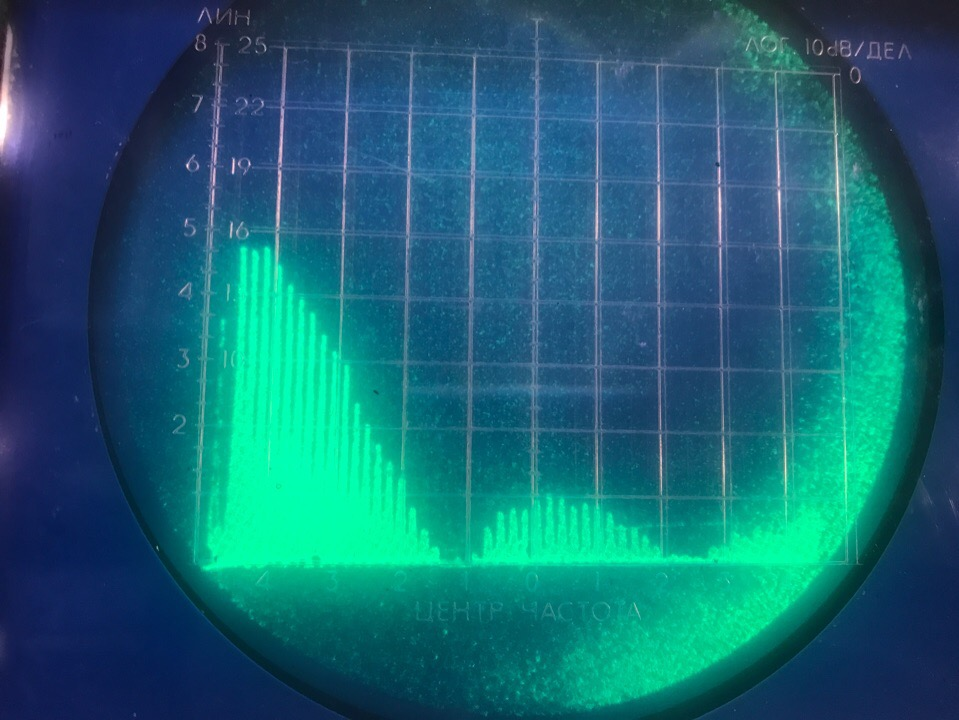
\includegraphics[scale=0.3]{2.jpg}
\caption{Спектр прямоугольных импульсов при $f_\text{повт} = 1$ кГц и $\tau = 50$ мкс}
\end{figure}
\begin{figure}[H]
\center
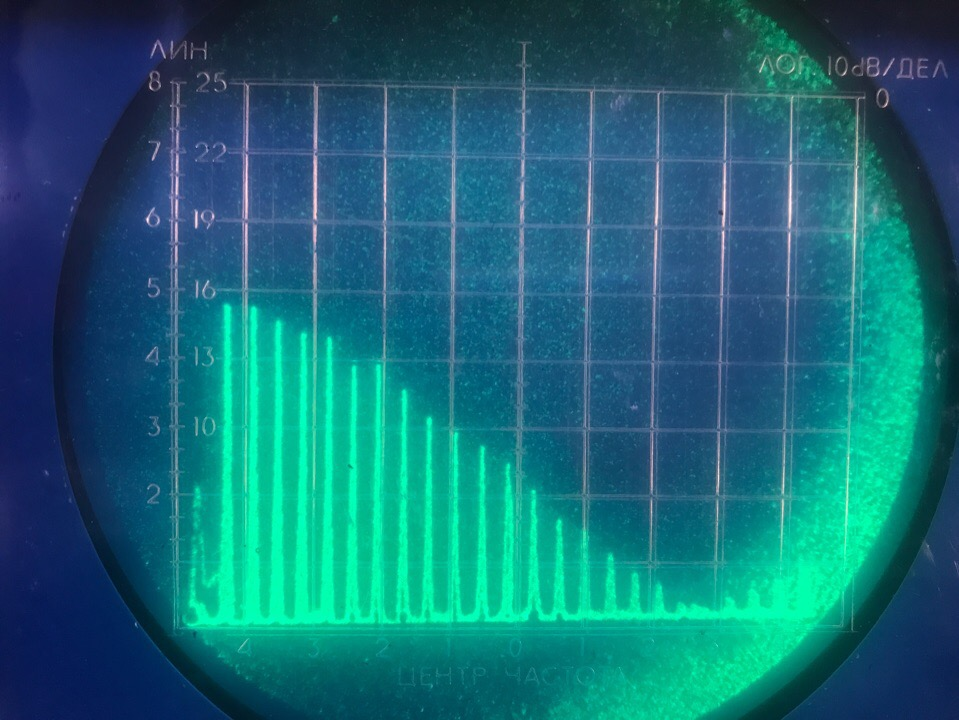
\includegraphics[scale=0.3]{3.jpg}
\caption{Спектр прямоугольных импульсов при $f_\text{повт} = 2$ кГц и $\tau = 50$ мкс}
\end{figure}
Построим график $\Delta \nu (1 / \tau)$:
\begin{figure}[H]
\center
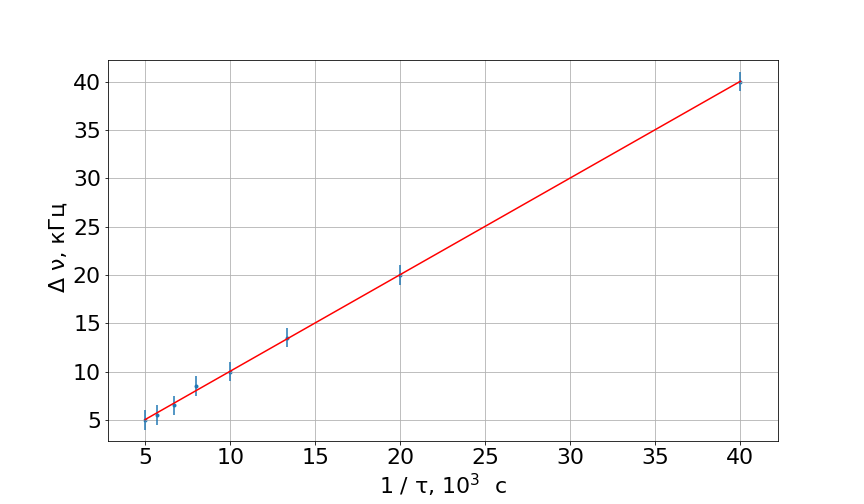
\includegraphics[scale=0.4]{gra1.png}
\caption{График зависимости $\Delta \nu$ от $1 / \tau$}
\end{figure}
Коэффициент угла наклона графика $k = 1 \Rightarrow$ с большой точностью выполняется соотношение неопределённостей.

\textbf{Исследование спектра периодической последовательности цугов гармонических колебаний:}
\begin{figure}[H]
\center
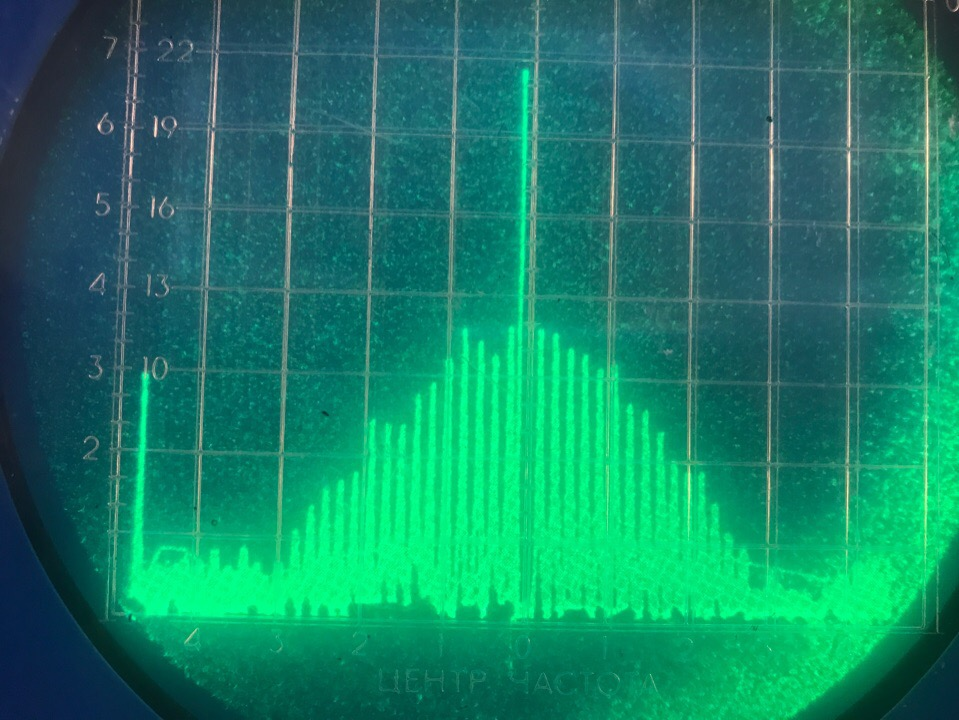
\includegraphics[scale=0.3]{4.jpg}
\caption{Спектр цугов при $f_\text{повт} = 1$ кГц и $\tau = 50$ мкс}
\end{figure}
\begin{figure}[H]
\center
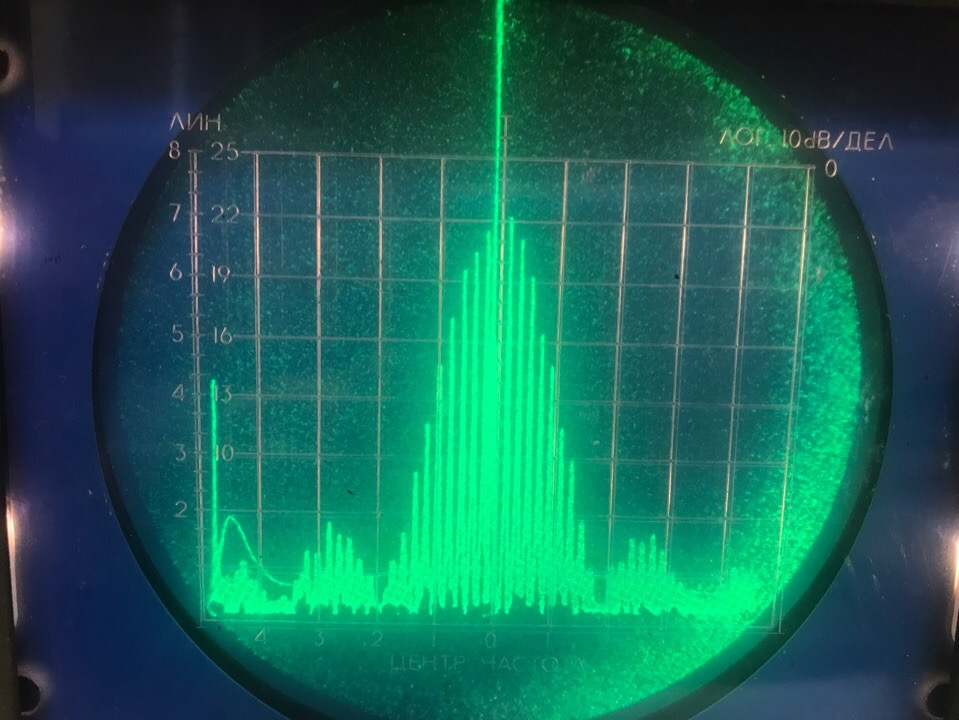
\includegraphics[scale=0.3]{5.jpg}
\caption{Спектр цугов при $f_\text{повт} = 1$ кГц и $\tau = 100$ мкс}
\end{figure}
\begin{figure}[H]
\center
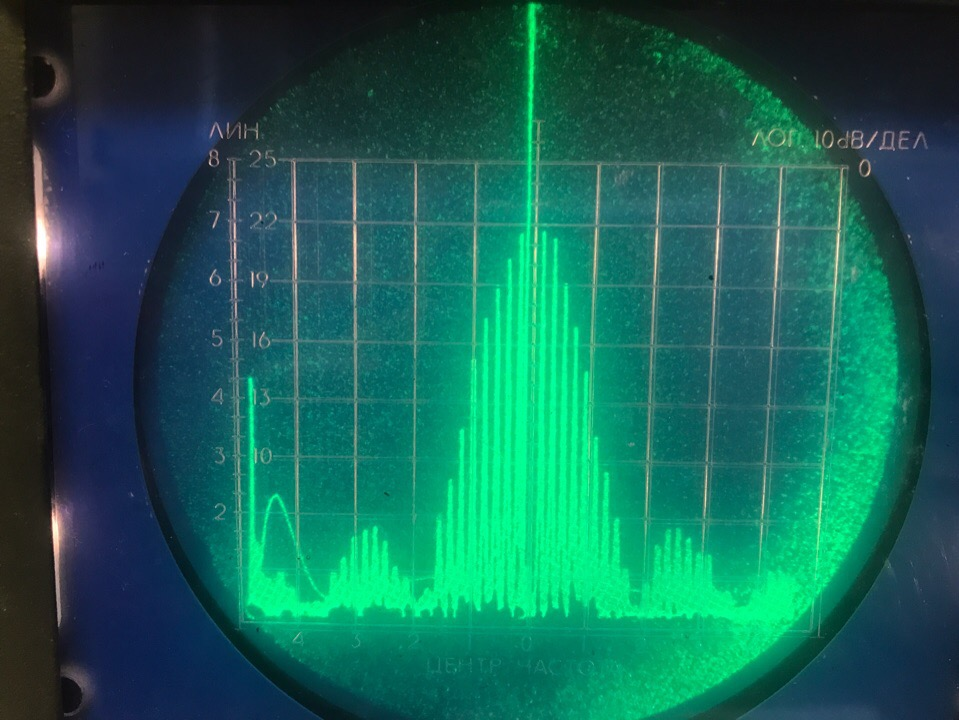
\includegraphics[scale=0.3]{6.jpg}
\caption{Спектр цугов при $\nu_0 = 25$ кГц и $\tau = 50$ мкс}
\end{figure}
\begin{figure}[H]
\center
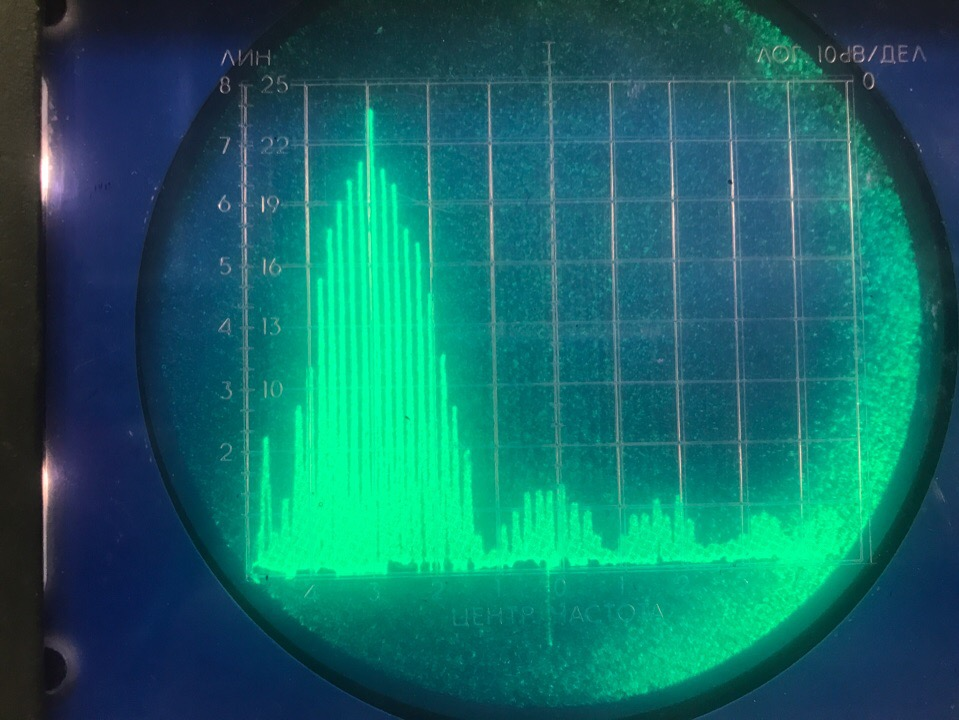
\includegraphics[scale=0.3]{7.jpg}
\caption{Спектр цугов при $\nu_0 = 10$ кГц и $\tau = 50$ мкс}
\end{figure}
Исследуем зависимость расстояния $\delta \nu$ между соседними спектральными компонентами от периода $T$ (частоты повторения импульсов $f_\text{повт}$ в диапазоне 1-8 кГц):
\begin{figure}[H]
\center
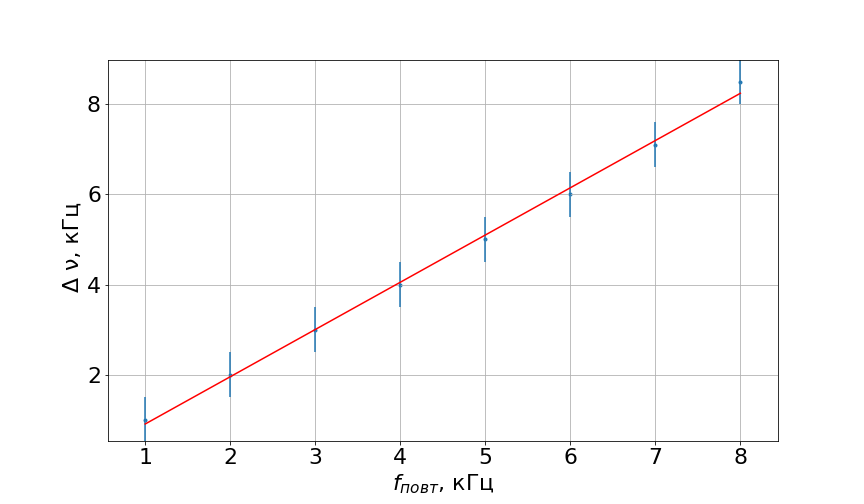
\includegraphics[scale=0.4]{gra2.png}
\caption{График зависимости $\Delta \nu$ от $f_\text{повт}$}
\end{figure}
Угловой наклон графика $k = 1.04$, что с достаточной точностью подтверждает справедливость соотношения неопределённости.
\textbf{Исследование спектра гармонических сигналов, модулированных по амплитуде}
Измеряя глубину модуляции, исследуем зависимость отношения амплитуды боковой линии спектра к амплитуде основной линии ($a_\text{бок} / a_\text{осн}$) от глубины модуляции $m$ и построим график:
\[
	m = \frac{A_{max} - A_{min}}{A_{max} + A_{min}}.
\]
\begin{figure}[H]
\center
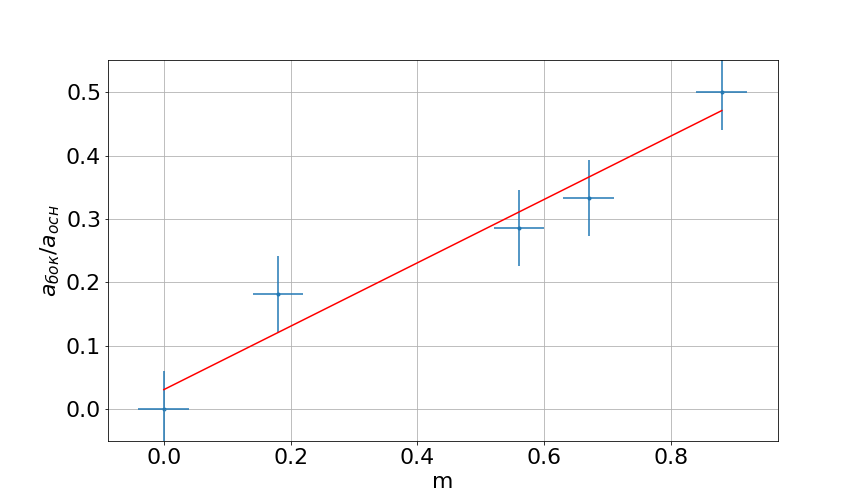
\includegraphics[scale=0.4]{gra3.png}
\caption{График зависимости $a_\text{бок} / a_\text{осн}$ от $m$}
\end{figure}
Угловой коэффициент наклона графика $k_\text{прак} = 0.5$. По формуле $a_\text{бок} = a_\text{осн} \cdot m / 2 \Rightarrow k_\text{теор} = 0.5$
\section*{Вывод}
В данной лабораторной работе мы исследовали соотношение неопределённости $\Delta \nu \cdot \tau \simeq 1$ --- несовместимость острой локализации волнового процесса во времени с узким спектром частот.
\end{document}